\documentclass[a4paper,11pt]{article}

\usepackage [french]{babel}
\usepackage [utf8]{inputenc}
\usepackage{graphicx}
\usepackage[T1]{fontenc}
\usepackage{textcomp}
\usepackage{vmargin}
\usepackage{dirtree}
\usepackage{listingsutf8}
\usepackage{xcolor}
\usepackage{textcomp}
\usepackage{float}
\usepackage{hyperref}
\usepackage{fancyhdr}
%\usepackage{fullpage}

\begin{document}

\lstset{
  inputencoding=utf8/latin1,
  belowcaptionskip=1\baselineskip,
  inputencoding=utf8/latin1,
  breaklines=true,
  language=C++,
  showstringspaces=false,
  basicstyle=\footnotesize\ttfamily,
  keywordstyle=\bfseries\color{purple!40!black},
  commentstyle=\itshape\color{green!40!black},
  identifierstyle=\color{black},
  stringstyle=\color{blue},
  morekeywords={QXmlStreamReader, QString, QTextCursor, QSyntaxHighLighter, QRegExp, XmlFileManager, QFile, QIODevice, QDomNode, QDomDocument, stack, ModeleXml, QStandardItem, QStandardItemModel, QModelIndex},
    showspaces=false,                % show spaces everywhere adding particular underscores; it overrides 'showstringspaces'
  showtabs=false,                  % show tabs within strings adding particular underscores
  stepnumber=2,                    % the step between two line-numbers. If it's 1, each line wil
  tabsize=2,                       % sets default tabsize to 2 spaces
  frame=lrtb,
  numbers=left
}

\title{\textbf{Imagerie 3D}\\Compte rendu TP2}
\author{\textit{\date\today Stéphane Wouters}}

\maketitle
\thispagestyle{empty}

\newpage 

\tableofcontents

\newpage 

\section{Architecture}
\paragraph{}

\subsection{Classe Voxel}

Un voxel est définit par son centre et par sa taille.

\begin{lstlisting}
class Voxel {

	Point center;
	float sizeX;
	float sizeY;
	float sizeZ;
	VALUE value;

	Voxel(float x, float y, float z, VALUE value) {
		this->value = value;
		center.set(x,y,z);
	}

	...
\end{lstlisting}

\subsection{Classe trianle}

Un voxel est définit par 3 coordonées

\begin{lstlisting}
class Triangle {
	
	Point p1;
	Point p2;
	Point p3;
	...
\end{lstlisting}

\subsection{Méthodes de la classe Voxel}

A partir d'un voxel, les méthodes suivantes sont définies :

\begin{itemize}
\item \bf{Point* getSommets()} Retourne la position des 8 sommets du voxel
\item \bf{Point* getAdj()} Retourne la position des 6 voxels adjacent (les centres)
\item \bf{Point* getTriangles(int numeroFace)} Retourne les deux triangle de la face numéro N (de 0 à 6)
\end{itemize}

\subsection{Alogrithme général}

La fonction retourne la liste des triangles générés.

\begin{lstlisting}
vector<Triangle> seuillage(Image img, int seuil) {

	vector<Triangle> out;

	// Parcours de l'image
	for (int i = 0; i < img.sizeX; ++i) {
		for (int j = 0; j < img.sizeY; ++j) {
			for (int k = 0; k < img.sizeZ; ++k) {

				// Calcul du voxel
				VALUE value = img.getValue(i,j,k);
				Voxel v(i,j,k, value);

				if (v.getValue() > seuil) {

					// Parcours des voisins
					for (auto adj : v.getAdj() {
						if (img.getValue(adj.x,adj.y,adj.z) < seuil) {

							// Calcul des triangles
							Triangle* triangles = v.getTriangles(face);
							out.push_back(triangles[0]);
							out.push_back(triangles[1]);
						}
					}
				}
			}
		}
	}
	return out;
}

\end{lstlisting}


\subsection{Ecriture dans fichier}

Pour retranscrire les triangles dans un fichier, on ajoute une méthode toString dans Triangle :

\begin{lstlisting}
string toString() {
	string s = "facet normal 0 0 0\n";
	s += "outer loop\n";
	s += "vertex "+p1.toString() +"\n";
	s += "vertex "+p2.toString() +"\n";
	s += "vertex "+p3.toString() +"\n";
	s += "endloop\nendfacet";
	return s;
}
\end{lstlisting}

On affiche toString() sur chacun des triangles de sortie, et on redirige la sortie standard vers un fichier STL à l'excutation du fichier binaire..

\section{Résultats}

\begin{figure}[H]
 \center
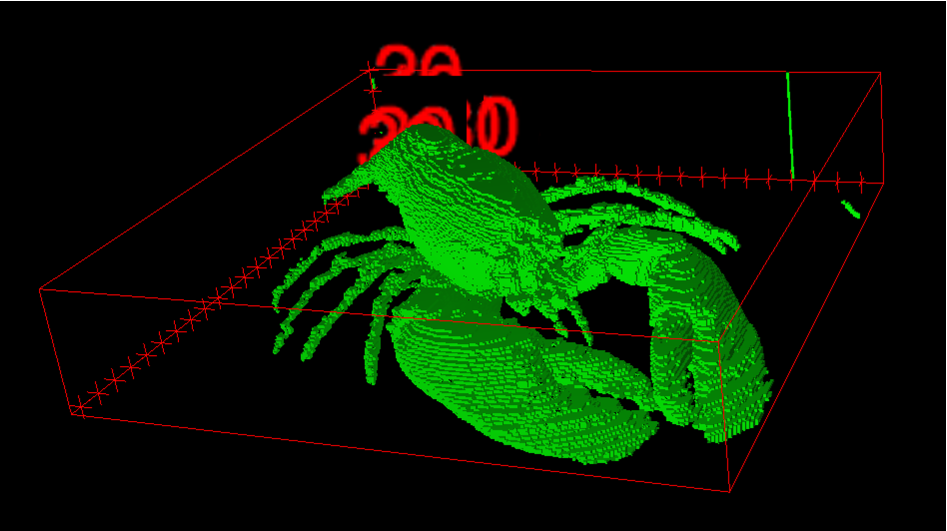
\includegraphics[scale=0.7]{homard_figi.png}
\caption{Whatisit sous FIGI}
\end{figure}

\begin{figure}[H]
 \center
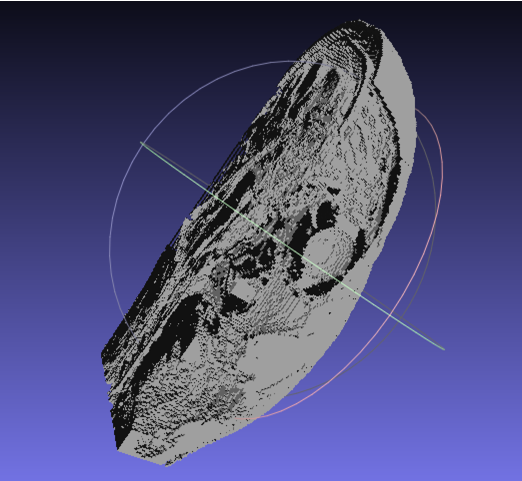
\includegraphics[scale=0.7]{brainix.png}
\caption{Brainix sous MeshLab}
\end{figure}

\begin{figure}[H]
 \center
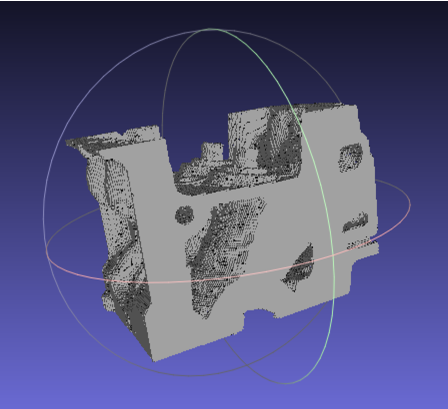
\includegraphics[scale=0.7]{egine_100_meshlab.png}
\caption{Engine, seuil 100 sous MeshLab}
\end{figure}

\begin{figure}[H]
 \center
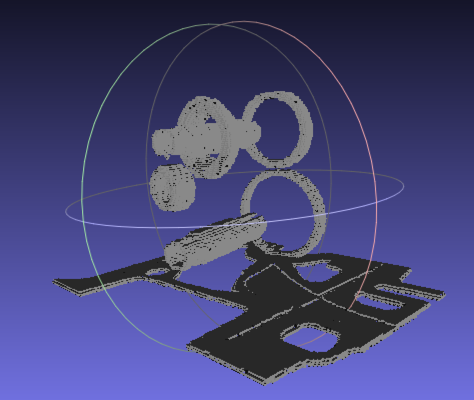
\includegraphics[scale=0.7]{engine_200_meshlab.png}
\caption{Engine, seuil 200 sous MeshLab}
\end{figure}

\paragraph{}

\section{Code source}

\subsection{Librairie}

\begin{lstlisting}
#ifndef VOXEL_PPM
#define VOXEL_PPM

#include <iostream>
#include <stdlib.h>
#include <stdio.h>
#include <string>
#include <math.h>
#include "Image.h"

typedef unsigned short VALUE;

using namespace std;

class Point {
public:
	float x;
	float y;
	float z;

	Point() {
		set(0,0,0);
	}

	Point(float x, float y, float z) {
		set(x,y,z);
	}

	void set(float x, float y, float z) {
		this->x = x;
		this->y = y;
		this->z = z;
	}

	string toString() {
		char s[250];
		sprintf(s, "%f %f %f", x, y, z);
		return s;
	}
};

class Triangle {
public:
	Point p1;
	Point p2;
	Point p3;

	string toString() {
		string s = "facet normal 0 0 0\n";
		s += "outer loop\n";
		s += "vertex "+p1.toString() +"\n";
		s += "vertex "+p2.toString() +"\n";
		s += "vertex "+p3.toString() +"\n";
		s += "endloop\nendfacet";
		return s;
	}

};


class Voxel {
public:

	Point center;
	float sizeX;
	float sizeY;
	float sizeZ;
	VALUE value;

	Voxel(float x, float y, float z, VALUE value) {
		this->value = value;
		center.set(x,y,z);
		sizeX = 1;
		sizeY = 1;
		sizeZ = 1;
	}

	Point* getSommets() {
		Point* sommets = new Point[8];
		sommets[0].set(center.x -sizeX/2, center.y -sizeY/2, center.z -sizeZ/2);
		sommets[1].set(center.x +sizeX/2, center.y -sizeY/2, center.z -sizeZ/2);
		sommets[2].set(center.x +sizeX/2, center.y +sizeY/2, center.z -sizeZ/2);
		sommets[3].set(center.x -sizeX/2, center.y +sizeY/2, center.z -sizeZ/2);
		sommets[4].set(center.x -sizeX/2, center.y -sizeY/2, center.z +sizeZ/2);
		sommets[5].set(center.x +sizeX/2, center.y -sizeY/2, center.z +sizeZ/2);
		sommets[6].set(center.x +sizeX/2, center.y +sizeY/2, center.z +sizeZ/2);
		sommets[7].set(center.x -sizeX/2, center.y +sizeY/2, center.z +sizeZ/2);
		return sommets;
	}

	// Numéro de la face de 0 à 5
	Triangle* getTriangles(int nFace) {
		Triangle* triangles = new Triangle[2];
		Point* sommets = getSommets();

		switch (nFace) {
			case 0: // Droite
				triangles[0].p1 = sommets[1];
				triangles[0].p2 = sommets[2];
				triangles[0].p3 = sommets[5];
				triangles[1].p1 = sommets[2];
				triangles[1].p2 = sommets[6];
				triangles[1].p3 = sommets[5];
				break;
			case 1: // Gauche
				triangles[0].p1 = sommets[4];
				triangles[0].p2 = sommets[3];
				triangles[0].p3 = sommets[0];
				triangles[1].p1 = sommets[4];
				triangles[1].p2 = sommets[6];
				triangles[1].p3 = sommets[3];
				break;
			case 2: // Derrière
				triangles[0].p1 = sommets[6];
				triangles[0].p2 = sommets[2];
				triangles[0].p3 = sommets[3];
				triangles[1].p1 = sommets[6];
				triangles[1].p2 = sommets[3];
				triangles[1].p3 = sommets[7];
				break;
			case 3: // Devant
				triangles[0].p1 = sommets[0];
				triangles[0].p2 = sommets[1];
				triangles[0].p3 = sommets[5];
				triangles[1].p1 = sommets[0];
				triangles[1].p2 = sommets[5];
				triangles[1].p3 = sommets[4];
				break;
			case 4: // Haut
				triangles[0].p1 = sommets[4];
				triangles[0].p2 = sommets[5];
				triangles[0].p3 = sommets[6];
				triangles[1].p1 = sommets[6];
				triangles[1].p2 = sommets[7];
				triangles[1].p3 = sommets[4];
				break;
			case 5: // Bas
				triangles[0].p1 = sommets[3];
				triangles[0].p2 = sommets[2];
				triangles[0].p3 = sommets[1];
				triangles[1].p1 = sommets[3];
				triangles[1].p2 = sommets[1];
				triangles[1].p3 = sommets[0];
				break;
		}
		
		return triangles;
	}

	Point* getAdj() {
		Point* voxels = new Point[6];
		voxels[0].set(center.x + 1, center.y, center.z);
		voxels[1].set(center.x - 1, center.y, center.z);
		voxels[2].set(center.x, center.y + 1, center.z);
		voxels[3].set(center.x, center.y - 1, center.z);
		voxels[4].set(center.x, center.y, center.z + 1);
		voxels[5].set(center.x, center.y, center.z - 1);
		return voxels;
	}

};


#endif


\end{lstlisting}

\subsection{Algorithme de seuillage}

\begin{lstlisting}
#ifndef IMAGETOOLS_PPM
#define IMAGETOOLS_PPM

#include <iostream>
#include <stdlib.h>
#include <stdio.h>
#include <string.h>
#include <math.h>
#include "Image.h"
#include "Voxel.h"
#include <Vector>

vector<Triangle> seuillage(Image img, int seuil) {

	vector<Triangle> out;

	for (int i = 0; i < img.sizeX; ++i) {
		for (int j = 0; j < img.sizeY; ++j) {
			for (int k = 0; k < img.sizeZ; ++k) {
				VALUE value = img.getValue(i,j,k);
				Voxel v(i,j,k, value);
				if (value > seuil) {
					Point* adjs = v.getAdj();
					for (int face = 0; face < 6; ++face) {
						Point adj = adjs[face];
						VALUE valueADJ = img.getValue(adj.x,adj.y,adj.z);
						if (valueADJ < seuil) {
							Triangle* triangles = v.getTriangles(face);
							out.push_back(triangles[0]);
							out.push_back(triangles[1]);
						}
					}
				}
			}
		}
	}
	return out;
}

void print(vector<Triangle> tab) {
	for (auto var : tab) {
		cout << var.toString() << endl;
	}
}
#endif
\end{lstlisting}

\subsection{Fichier main}
\begin{lstlisting}
#include "../lib/Image.h"
#include "../lib/Voxel.h"
#include "../lib/ImageTools.h"
#include <iostream>
#include <algorithm>

using namespace std;

void printModel(const char* path, int seuil, int sizeX, int sizeY, int sizeZ) {
	Image in(sizeX, sizeY, sizeZ);
	in.load(path);
	cout << "solid name" << endl;
	vector<Triangle> triangles = seuillage(in, seuil);
	print(triangles);
	cout << "endsolid name" << endl;
}

int main() {
	//printModel("../ressources/BRAINIX/brainix.256x256x100.0.9375x0.9375x1.5.img", 200, 256, 256, 100);
	printModel("../ressources/MANIX/manixSansIV.512x512x48.0.4570x0.4570x3.0.img", 1250, 512, 512, 48);
	//printModel("../ressources/BEAUFIX/beaufix.448x576x72.0.6250x0.6250x1.4.img", 120, 576, 72, 448);
	//printModel("../ressources/WHATISIT/whatisit.301x324x56.1.1.1.4.img", 50, 301, 324, 56);
	//printModel("../ressources/engine/engine.256x256x128.1x1x1.img", 200, 256, 256, 128);
}
\end{lstlisting}


\end{document}

